% !TeX root = ../../../main.tex
\subsubsection{Additional Sensitivity Analyses}
\label{ch05:sec:additional-sensitivity-analyses}

\ChFiveHeadingOnly
\paragraph{Varying the Event Match Distance Threshold}

We conducted sensitivity analyses to assess robustness with respect to the event match threshold.
As expected, stricter thresholds produce fewer but cleaner matches, while more permissive thresholds increase coverage at the expense of noisier ordering and timing.
Varying the cosine distance threshold from \ChFiveRebuttal{0.01 to 0.50 (in increments of 0.01 for both the recursive and LAPJV matching analyses)}, we observed corresponding shifts in event match recall, concordance, and AULTC.
A threshold of 0.10 was chosen based on manual review of \texttt{Llama 3.3 70B Instruct} and \texttt{O1} outputs.
The resulting trade-offs are summarized in Figure~\ref{ch05:fig:threshold_tradeoff_greedy}.



Similarly, LAPJV preserves high event match rates at low thresholds across models and exhibits a smooth trade-off between coverage and temporal accuracy (Supplementary Material, Section \ref{ch05:apd:lapjv-matching} Figure~\ref{ch05:fig:threshold_tradeoff_LAPJV}).
The resulting operating points are highly comparable to those obtained using the recursive matching heuristic.
In particular, the heuristic matcher yields slightly stronger concordance near the elbow of the trade-off curve, while LAPJV achieves marginally higher AULTC values, reflecting improved timestamp alignment under global assignment.
Overall, both strategies lead to consistent qualitative conclusions.

\ChFiveRebuttal{For both Figure~\ref{ch05:fig:threshold_tradeoff_greedy} and Figure~\ref{ch05:fig:threshold_tradeoff_LAPJV}, model trajectories change smoothly in the neighborhood of 0.1, but the rank
order is not invariant across the full threshold range, particularly for AULTC where several curves are close or cross.
We therefore interpret the curves as coverage-versus-temporal-accuracy trade-offs rather than evidence of one
threshold-independent winner.}


\paragraph{Sensitivity to Parts of the LLM Prompt Being Changed}
We conducted sensitivity analyses to assess how different components of the extraction prompt affect timeline quality (Supplementary Material, Section~\ref{ch05:apd:sensitivity-llm-prompt}).
Structured prompts that include explicit temporal instructions (e.g., Interval and Interval+Type) consistently improved semantic alignment, temporal ordering, and timestamp accuracy.
In contrast, removing role framing or conjunction expansion led to modest degradation, and Zero-shot prompting performed substantially worse across all metrics.
These results highlight that prompt design plays an important role in guiding LLMs to produce high-quality temporal annotations (Figure~\ref{ch05:fig:prompt_ablation}).



% !TeX root = ../../../main.tex
\begin{figure}[htbp]
\begin{ChFiveFloatBody}
\centering
        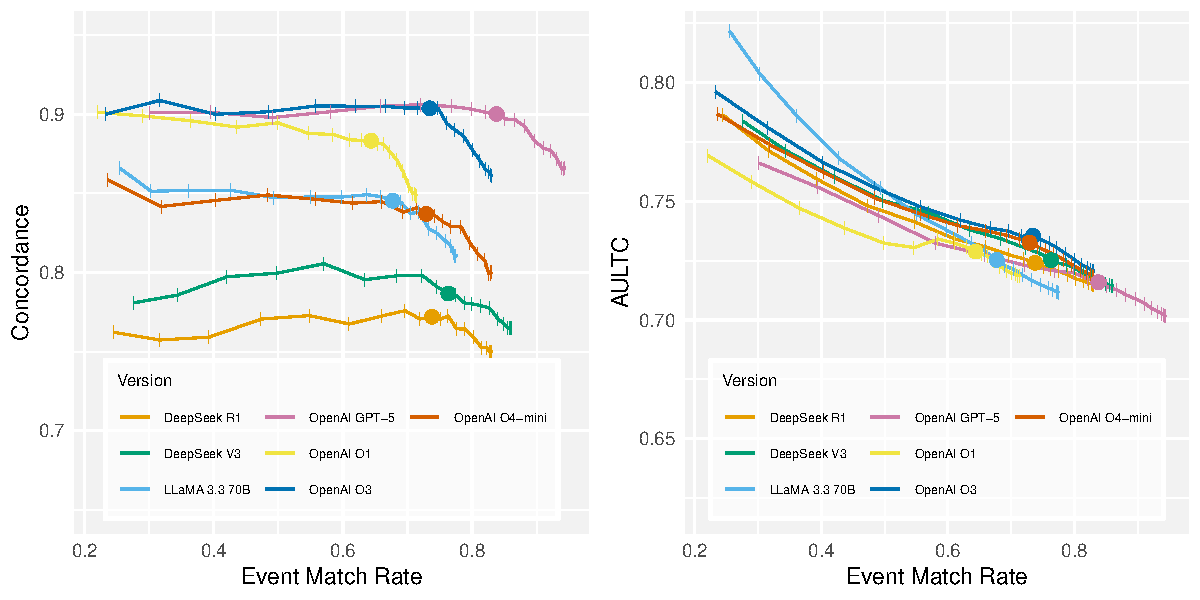
\includegraphics[width=\linewidth]{Chapters/chapter-05/images/Scientific_data/Plots_tables/event_match_vs_metrics_updated.pdf}

    
    
    

\end{ChFiveFloatBody}
\caption{Concordance and AULTC by event match rate for recursive matching heuristic. Solid circle ($\bullet$) represents threshold of 0.1, with ticks (|) indicating 0.01 increments of the threshold in [0.01, 0.50].
    }\ChFiveFloatLabel{ch05:fig:threshold_tradeoff_greedy}
\end{figure}





\paragraph{Inter-LLM comparison of temporal annotations}
Finally, we qualitatively compared temporal annotations produced by several LLMs on a representative case report to illustrate characteristic differences in event extraction and timestamping (Supplementary Material, Section~\ref{ch05:apd:inter-llm-comparison}, Figure~\ref{ch05:fig:tts_evaluation}).
While all models recovered the major clinical trajectory and preserved temporal polarity, they varied in
event granularity, paraphrasing, and long-range temporal normalization.
These differences complement the aggregate quantitative results and highlight the impact of model behavior on the structure of extracted timelines.
Common model-specific error patterns, such as granularity variation, duplicate events, and differences in temporal normalization, are summarized in the Supplementary Material, Section~\ref{ch05:apd:inter-llm-comparison}, Table~\ref{ch05:tab:error_taxonomy}.

\paragraph{Validation of Structured Fields}
\label{ch05:sec:structured-field-validation}

\ChFiveRebuttal{
We manually validated the structured fields on 88 confirmed case reports of \texttt{case\_study\_100} split. Across 264 demographic fields, 247 were correct (93.6\%): age accuracy was 95.5\% (84/88), sex accuracy was 97.7\% (86/88), and ethnicity accuracy was 87.5\% (77/88). Of 517 extracted diagnosis entries, 505 were supported by the source report, corresponding to 97.7\% precision. After revising the UMLS-linking procedure, 478/517 diagnosis mappings (92.46\%) were judged acceptable and 39/517 (7.54\%) incorrect.
}

\ChFiveRebuttal{
Demographic errors were concentrated in missing or malformed values; diagnosis errors primarily reflected family history, excluded differentials, or hypothetical complications assigned to the patient. UMLS errors most often involved an inappropriate semantic type or an overly generic concept.
}


